\documentclass{article}
\usepackage[T1]{fontenc}
\usepackage{lmodern}
\usepackage{graphicx}
\usepackage{amsmath,amssymb}
\usepackage[a4paper,margin=2cm]{geometry}
\usepackage[absolute,overlay]{textpos}
\setlength{\TPHorizModule}{1mm}
\setlength{\TPVertModule}{1mm}
\usepackage[indonesian]{babel}
\usepackage{hyperref}
\setlength{\emergencystretch}{2em}
% unit: Halaman 69

\begin{document}

% === Halaman 69 (llm) ===

\textbf{Running program:}

\vspace{170.77mm}

>> LSB\_sisip\nKetikkan nama file citra cover: peppers.bmp\nKetikkan pesan: Mari kita jaga negara kesatuan Republik Indonesia tercinta. Oke?\nPenyisipan pesan....\nKetikkan nama file citra stego (bmp): output.bmp\nSelesai\n>>

% deskripsi: Screenshot jendela program yang menampilkan 'Citra cover' berisi gambar paprika warna-warni.
% bbox normalisasi: [0.1270, 0.4080, 0.4360, 0.9830]
\begin{textblock*}{64.89mm}(26.67mm,121.18mm)
\noindent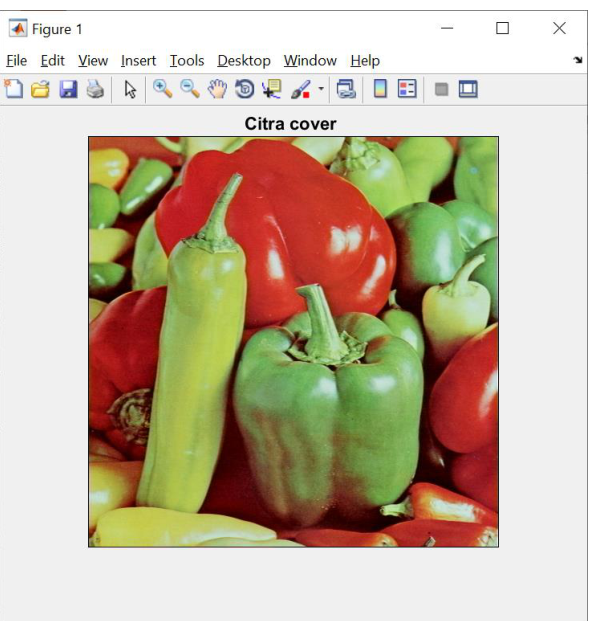
\includegraphics[width=64.89mm,height=170.77mm]{../../images/llm/page_069_img_01.png}%
\end{textblock*}

% deskripsi: Screenshot jendela program yang menampilkan 'Citra stego' berisi gambar paprika yang secara visual terlihat identik dengan citra cover.
% bbox normalisasi: [0.5030, 0.4080, 0.8320, 0.9830]
\begin{textblock*}{69.09mm}(105.63mm,121.18mm)
\noindent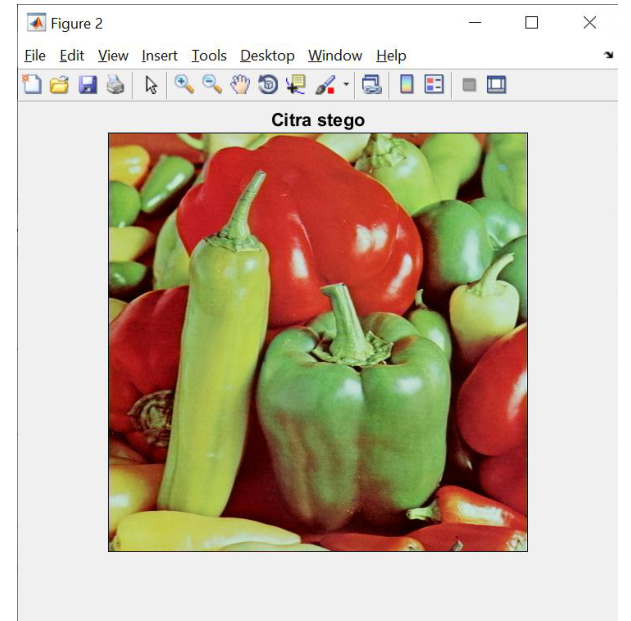
\includegraphics[width=69.09mm,height=170.77mm]{../../images/llm/page_069_img_02.png}%
\end{textblock*}

\end{document}
